\documentclass[sigconf, nonacm]{acmart}

%%% VLDB block start %%%
\usepackage{pvldb}
%%% VLDB block end %%%
\renewcommand\vldbdoi{XX.XX/XXX.XX}
\renewcommand\vldbpages{XXX-XXX}
\renewcommand\vldbavailabilityurl{https://github.com/WanderingSnail/semlake_milestone2}

\usepackage{booktabs}
\usepackage{multirow}
\usepackage{algorithm}
\usepackage[noend]{algpseudocode}
\usepackage{tikz}
\usetikzlibrary{arrows.meta,positioning,calc}

\newcommand{\sys}{\textsc{SemLake}}
\newtheorem{assumption}{Assumption}
\algrenewcommand\algorithmicindent{0.9em}

%% Every number below comes from benchmarks/results/ through benchmarks/paper_numbers.py.
% Generated by benchmarks/paper_numbers.py from benchmarks/results/. Do not edit.
\newcommand{\BenchLines}{4{,}700}
\newcommand{\BoneRSelAtOne}{1.00}
\newcommand{\BoneRSuiteFP}{6}
\newcommand{\BoneRSuitePrec}{0.65}
\newcommand{\BoneRSuiteRec}{0.79}
\newcommand{\BoneRSuiteTP}{11}
\newcommand{\BoneRTpchFP}{3}
\newcommand{\BoneRTpchPrec}{0.88}
\newcommand{\BoneRTpchRec}{1.00}
\newcommand{\BsixSuiteFP}{0}
\newcommand{\BsixSuitePrec}{--}
\newcommand{\BsixSuiteRec}{0.00}
\newcommand{\BsixSuiteTP}{0}
\newcommand{\BsixTpchFP}{0}
\newcommand{\BsixTpchPrec}{--}
\newcommand{\BsixTpchRec}{0.00}
\newcommand{\CostBtwo}{\$0.228}
\newcommand{\CostSemLoc}{\$0.086}
\newcommand{\CostSemUni}{\$0.088}
\newcommand{\CrossLoc}{3{,}094}
\newcommand{\CrossUni}{446}
\newcommand{\DoltSuiteFP}{0}
\newcommand{\DoltSuitePrec}{1.00}
\newcommand{\DoltSuiteRec}{0.14}
\newcommand{\DoltSuiteTP}{2}
\newcommand{\DoltTpchFP}{0}
\newcommand{\DoltTpchPrec}{--}
\newcommand{\DoltTpchRec}{0.00}
\newcommand{\DuckdbVersion}{1.5.6}
\newcommand{\EngineLines}{2{,}100}
\newcommand{\FuzzSeeds}{200}
\newcommand{\HistHigh}{360}
\newcommand{\HistLca}{3.5 and 6.6}
\newcommand{\HistLow}{42}
\newcommand{\HistSemHigh}{1.20}
\newcommand{\HistSemLow}{0.53}
\newcommand{\MachineCores}{4}
\newcommand{\PackBoneMax}{1.00}
\newcommand{\PackChanged}{4}
\newcommand{\PackMax}{1{,}024}
\newcommand{\PackRows}{1{,}024}
\newcommand{\PyarrowVersion}{26.0.0}
\newcommand{\PythonVersion}{3.13.16}
\newcommand{\Repeats}{5}
\newcommand{\ScanGroupRows}{100{,}000}
\newcommand{\ScanGroups}{61}
\newcommand{\ScanLocHigh}{+6.9}
\newcommand{\ScanLocLow}{$-$3.4}
\newcommand{\ScanLocOver}{+0.9}
\newcommand{\ScanRows}{6{,}100{,}000}
\newcommand{\ScanUniOver}{+6.0}
\newcommand{\SelMaxPct}{20}
\newcommand{\SelMinPct}{0.019}
\newcommand{\SelQsixFiles}{6}
\newcommand{\SelTrials}{12}
\newcommand{\SemSelMax}{0.00}
\newcommand{\SemSuiteFP}{0}
\newcommand{\SemSuitePrec}{1.00}
\newcommand{\SemSuiteRec}{1.00}
\newcommand{\SemSuiteTP}{14}
\newcommand{\SemTpchFP}{0}
\newcommand{\SemTpchPrec}{1.00}
\newcommand{\SemTpchRec}{1.00}
\newcommand{\StaticSelMean}{0.67}
\newcommand{\StaticSuiteFP}{2}
\newcommand{\StaticSuitePrec}{0.88}
\newcommand{\StaticSuiteRec}{1.00}
\newcommand{\StaticSuiteTP}{14}
\newcommand{\StaticTpchFP}{8}
\newcommand{\StaticTpchPrec}{0.73}
\newcommand{\StaticTpchRec}{1.00}
\newcommand{\SuiteCases}{27}
\newcommand{\SuitePos}{14}
\newcommand{\SwarmBoneHazTotal}{63}
\newcommand{\SwarmBoneRFBThirtyTwo}{19.6}
\newcommand{\SwarmBoneRHazTotal}{27}
\newcommand{\SwarmBtwoHazTotal}{9}
\newcommand{\SwarmDeletePct}{5}
\newcommand{\SwarmFiles}{32}
\newcommand{\SwarmGroup}{8}
\newcommand{\SwarmGroupSixtyFour}{17.1}
\newcommand{\SwarmHeavyAgents}{8 and 32}
\newcommand{\SwarmHeavyDeletePct}{15}
\newcommand{\SwarmHeavyReportPct}{30}
\newcommand{\SwarmHorizon}{60}
\newcommand{\SwarmMaxAgents}{64}
\newcommand{\SwarmReportPct}{15}
\newcommand{\SwarmRowsPerFile}{32}
\newcommand{\SwarmRtt}{10}
\newcommand{\SwarmSeeds}{5}
\newcommand{\SwarmSemFBThirtyTwo}{0.2}
\newcommand{\SwarmSemHazTotal}{0}
\newcommand{\SwarmSemSixtyFour}{4.8}
\newcommand{\SwarmUpdatePct}{80}
\newcommand{\SwarmWorkMean}{2}
\newcommand{\TpchFiles}{31}
\newcommand{\TpchPairs}{42}
\newcommand{\TpchPos}{22}
\newcommand{\TpchRows}{60{,}175}
\newcommand{\TpchSF}{0.01}
\newcommand{\WfourBoneTen}{147.0}
\newcommand{\WfourBthreeReq}{20{,}009}
\newcommand{\WfourBthreeTen}{171.4}
\newcommand{\WfourBtwoTen}{129.8}
\newcommand{\WfourSemOne}{0.38}
\newcommand{\WfourSemTen}{3.22}
\newcommand{\WoneSBtwoEst}{1{,}301}
\newcommand{\WoneSBytesSem}{380}
\newcommand{\WoneSFilesK}{10}
\newcommand{\WoneSGetSem}{3}
\newcommand{\WoneSListSem}{1}
\newcommand{\WoneSPutSem}{3}
\newcommand{\WoneSReqBone}{5}
\newcommand{\WoneSReqBtwo}{20{,}007}
\newcommand{\WoneSReqSem}{7}
\newcommand{\WtwoBfourZero}{37.9}
\newcommand{\WtwoBoneEst}{0.48}
\newcommand{\WtwoBoneTwenty}{203.2}
\newcommand{\WtwoBoneZero}{227.3}
\newcommand{\WtwoSemEst}{0.55}
\newcommand{\WtwoSemTwenty}{8.12}
\newcommand{\WtwoSemZero}{9.02}


\begin{document}
\title{SemLake: Predicate-Level Three-Way Merge for Branched Data Lakehouses}

\author{Xiaofan Cao}
\email{xc2314895@qu.edu.qa}

\begin{abstract}
Lakehouse catalogs such as lakeFS, Nessie and Bauplan let a pipeline fork a table in milliseconds, but merging two branches back is decided by physical overlap: which files, or which rows, both branches wrote. This rule is wrong in both directions. Two branches that update different rows of the same Parquet file conflict under file-level optimistic concurrency control, and a compliance purge on one branch merges silently with a report on the other that aggregated the purged rows, because the two branches wrote disjoint files. We present \sys, a three-way merge for branched lakehouse tables that decides conflicts on what each branch read and deleted. Each commit stores a small summary with its row changes, the pre-images of deleted rows, and the \texttt{WHERE} clauses of its reads and deletes. A merge replays only the summaries written since the fork, tests read and delete clauses for overlap with a static satisfiability check over a conjunctive fragment, and falls back to evaluating the read clause on the deleted rows' recorded values. Rows changed by both branches are combined by column; true cell collisions are kept as explicit choices. The merged snapshot is written as deletion-vector updates and one delta file, so no base file is rewritten. On \SuiteCases\ labelled merge scenarios, \sys\ reaches recall \SemSuiteRec\ and precision \SemSuitePrec; Dolt reaches recall \DoltSuiteRec, and a model of Delta Lake's row-level checks reaches precision \BoneRSuitePrec. On \TpchPairs\ refresh-versus-query pairs over real TPC-H \texttt{lineitem}, \sys\ reaches recall \SemTpchRec\ and precision \SemTpchPrec. A merge on a \WoneSFilesK K-file table issues \WoneSReqSem\ object-store requests, against \WoneSReqBtwo\ for copy-on-write. In a simulated swarm of up to \SwarmMaxAgents\ agents committing to one table, \sys\ committed no hazards over \SwarmSeeds\ seeds, against \SwarmBoneHazTotal\ for file-level concurrency control.
\end{abstract}

\maketitle

%%% VLDB block start %%%
\vldbtopmatter
%%% VLDB block end %%%

%%%%%%%%%%%%%%%%%%%%%%%%%%%%%%%%%%%%%%%%%%%%%%%%%%%%%%%%%%%%%%%%%%%%%%%%%%%%%%%%
\section{Introduction}
\label{sec:intro}

Lakehouse tables keep their data in immutable Parquet files on object storage and describe each version of the table with a snapshot of metadata~\cite{armbrust2020delta,zaharia2021lakehouse,iceberg2025v3}. Because a snapshot is only metadata, a table can be branched by copying a pointer. lakeFS~\cite{lakefs} and Nessie~\cite{nessie} use this to give data pipelines Git-like branches: a write-audit-publish job, a backfill or a regulatory purge runs on its own branch and is merged into \texttt{main} when it is done. Agent frameworks are starting to do the same for AI agents that work on shared data~\cite{git4data2026,zhou2026chronos}.

Branching is cheap; merging is where the semantics live, and today it is decided by physical overlap. Iceberg and Delta Lake reject a commit when a concurrent commit changed a file it also changed~\cite{armbrust2020delta,iceberg2025v3}. Delta Lake's row-level concurrency narrows write conflicts to rows, but still rejects a transaction when a concurrent commit deleted rows from a file it read~\cite{deltaconcurrency}. Version-controlled databases such as Dolt merge at cell granularity and check declared constraints~\cite{dolt2026}. None of these rules looks at what a branch actually depended on, and each fails in one direction or the other (Figure~\ref{fig:motivating}):
\begin{itemize}
  \item \emph{False conflicts.} Two branches that update different rows of the same 128\,MB file conflict under file-level concurrency control. A row-level variant avoids the write conflict, but a report that scanned the file is still rejected when the other branch deletes one unrelated row from it.
  \item \emph{Silent corruption.} A purge branch deletes the VIP customers while a report branch computes revenue over the VIP customers and writes it to a new file. The two branches wrote disjoint files and disjoint rows, so every physical rule merges them. The merged table now publishes a figure derived from rows it claims to have erased.
\end{itemize}

\begin{figure}[t]
\centering
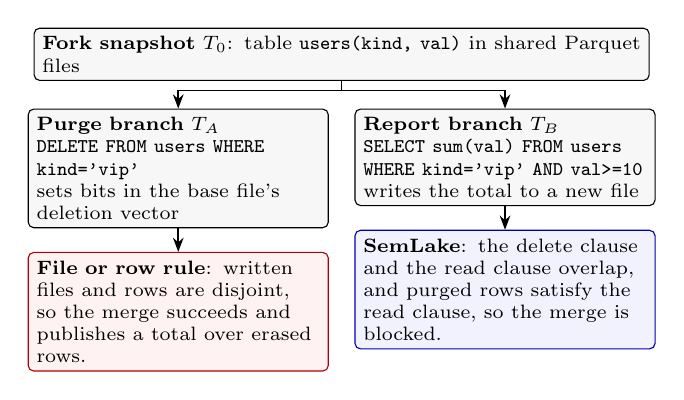
\begin{tikzpicture}[font=\scriptsize,
    box/.style={draw, rounded corners=2pt, align=left, inner sep=3pt, fill=gray!6},
    bad/.style={draw=red!70!black, rounded corners=2pt, align=left, inner sep=3pt, fill=red!5},
    good/.style={draw=blue!70!black, rounded corners=2pt, align=left, inner sep=3pt, fill=blue!5},
    arr/.style={-{Stealth[length=1.8mm]}, semithick}]
\node[box, text width=7.6cm] (base) {\textbf{Fork snapshot $T_0$}: table \texttt{users(kind, val)} in shared Parquet files};
\node[box, text width=3.6cm, below left=0.35cm and -3.75cm of base] (a) {\textbf{Purge branch $T_A$}\\\texttt{DELETE FROM users WHERE kind='vip'}\\sets bits in the base file's deletion vector};
\node[box, text width=3.6cm, below right=0.35cm and -3.75cm of base] (b) {\textbf{Report branch $T_B$}\\\texttt{SELECT sum(val) FROM users WHERE kind='vip' AND val>=10}\\writes the total to a new file};
\node[bad, text width=3.6cm, below=0.3cm of a] (x) {\textbf{File or row rule}: written files and rows are disjoint, so the merge succeeds and publishes a total over erased rows.};
\node[good, text width=3.6cm, below=0.3cm of b] (y) {\textbf{\sys}: the delete clause and the read clause overlap, and purged rows satisfy the read clause, so the merge is blocked.};
\draw[arr] (base.south) -- ++(0,-0.12) -| (a.north);
\draw[arr] (base.south) -- ++(0,-0.12) -| (b.north);
\draw[arr] (a) -- (x); \draw[arr] (b) -- (y);
\end{tikzpicture}
\caption{A purge and a report that touch disjoint files and rows. Physical merge rules accept the pair; \sys\ rejects it from commit metadata.}
\label{fig:motivating}
\end{figure}

Program-merge research has long treated three-way merge as a semantic question, with verified merges~\cite{sousa2018verified} and explicit representations of conflicting candidates~\cite{zhu2018conflict}. Those techniques reason about programs. A lakehouse merge must instead reason about which rows two branches read and removed, without scanning data files, because each object-store request costs tens of milliseconds and is billed~\cite{durner2023exploiting,s3pricing}.

\sys\ is a three-way merge for branched lakehouse tables built on that idea. Each commit writes a compact summary: its row changes, the values each deleted row had, and the \texttt{WHERE} clauses of the statements that read or deleted rows. A merge finds the fork point, replays the summaries written since then on each side, and checks every delete on one side against every read on the other. A static satisfiability test over a conjunctive fragment rules out most pairs at once; for the rest, the read clause is evaluated on the recorded values of the deleted rows. Rows changed by both sides are combined column by column, and a cell both sides set to different values is kept as an explicit choice. The merged snapshot is published with deletion vectors and a single delta file, so the merge touches only metadata and the changed rows.

This paper makes four contributions:
\begin{enumerate}
  \item A merge model for branched tables with four criteria, one per workload class, and the \emph{purge-safety} invariant for reads and deletes. We show that purge-safety and the serializability that SSI enforces are incomparable, and that purge-safety is the stricter of the two on read--delete pairs (Section~\ref{sec:model}).
  \item A conflict check that combines a static clause test with a check of the deleted rows' recorded values, and a replay of commit summaries since the fork that stays correct across chains of earlier merges. We prove that a merge the check accepts is purge-safe (Sections~\ref{sec:design} and~\ref{sec:correctness}).
  \item A merge that publishes deletion-vector updates and one delta file, with request counts that depend on the branch delta rather than on the table size (Section~\ref{sec:design_physical}).
  \item A prototype and an evaluation against file-level concurrency control, a model of Delta Lake's row-level checks, copy-on-write, tuple versioning, a CRDT merge, Dolt and an SSI model, on labelled scenarios, real TPC-H data and a simulated agent swarm (Sections~\ref{sec:impl} and~\ref{sec:eval}).
\end{enumerate}

%%%%%%%%%%%%%%%%%%%%%%%%%%%%%%%%%%%%%%%%%%%%%%%%%%%%%%%%%%%%%%%%%%%%%%%%%%%%%%%%
\section{Background and Problem}
\label{sec:background}

\subsection{Lakehouse Tables and Deletion Vectors}
A lakehouse table is a set of immutable Parquet files plus a metadata log; each commit produces a snapshot that lists the live files~\cite{armbrust2020delta,iceberg2025v3}. Files are large: Iceberg's default target is 512\,MB~\cite{icebergconfig}. Updating one row by copy-on-write therefore rewrites a whole file. Merge-on-read avoids this: a \emph{deletion vector} (DV), a Roaring bitmap~\cite{lemire2018roaring} attached to a data file, marks the positions of deleted or superseded rows, and new row versions go to a small delta file~\cite{okolnychyi2024petabyte,iceberg2025v3,delta2024rowlevel}. Readers skip masked positions, and compaction later folds the DVs back into clean files. Object stores charge per request and add tens of milliseconds per round trip~\cite{durner2023exploiting,s3pricing}, so the number of requests a merge issues matters as much as its CPU time.

\subsection{Workloads and Metrics}
\label{sec:bg_taxonomy}
Two branches $T_A$ and $T_B$ fork from a snapshot $T_0$ and are merged into $T_M$. We use four workload classes, each named by what the two branches do:
\begin{description}
  \item[W1, shared-file updates.] The branches update or delete different rows that live in the same files.
  \item[W2, hot rows.] The branches update overlapping rows; a fraction $\kappa$ of the changed rows is shared.
  \item[W3, read--delete dependencies.] One branch deletes rows that the other branch read to compute a result, or that it requires to stay live (a foreign-key parent, a row it cites), or it writes values that break a value rule the other branch declared.
  \item[W4, schema and scale.] One branch changes the schema while the other appends data; the table has many files and a deep commit history.
\end{description}
We measure four properties:
\begin{description}
  \item[M1, correctness.] Recall and precision of conflict detection on W3 and W4, and the false-abort rate on W1.
  \item[M2, merge latency.] CPU time of the merge, and the end-to-end time once object-store round trips are added, as the table, the history and $\kappa$ grow.
  \item[M3, object-store cost.] Requests and bytes written per merge, and dollars per 1,000 merges.
  \item[M4, read overhead.] The extra time of an analytical scan over a merged snapshot whose DVs have not been compacted.
\end{description}
Section~\ref{sec:eval_swarm} adds a fifth workload, a swarm of agents that branch from and commit to one table, and reports commit throughput for it.

\subsection{Existing Merge Rules}
\label{sec:baselines}
Table~\ref{tab:baselines} lists the rules we compare against. B1, B1R, B2 and B6 are decision rules that we implement over the same snapshots as \sys; B3 and B4 are merge strategies from the dataset-versioning and replicated-data literature that we reimplement; B5 is the Dolt binary.
\begin{description}
  \item[B1, file-level OCC.] The default of Iceberg and Delta Lake~\cite{armbrust2020delta,iceberg2025v3}: two commits conflict if they changed a common file.
  \item[B1R, Delta-style row-level checks.] Same-row writes conflict; a commit also conflicts when a concurrent commit deleted or changed rows in a file it read (\texttt{Concurrent\-Delete\-Read\-Exception}~\cite{deltaconcurrency}). We model B1R in its best case for data skipping, in which a branch reads only the files that contain at least one row matching its filter.
  \item[B2, row-level copy-on-write.] Rows are merged by identifier, as in copy-on-write tables, and every changed file is rewritten.
  \item[B3, tuple versioning.] Per-file version dictionaries in the style of Decibel and OrpheusDB~\cite{maddox2016decibel,huang2017orpheusdb}.
  \item[B4, CRDT merge.] Last-writer-wins per cell, as in conflict-free replicated views~\cite{faria2025crdv,almeida2024crdt}.
  \item[B5, Dolt.] Cell-level merge with declared \texttt{FOREIGN KEY} and \texttt{CHECK} constraints~\cite{dolt2026}.
  \item[B6, SSI.] Each branch is one transaction on $T_0$; the merge fails only if read--write dependencies run in both directions, as in serializable snapshot isolation~\cite{cahill2008serializable}, and same-row writes fail.
\end{description}

\begin{table}[t]
\centering
\footnotesize
\caption{What each merge rule compares, and how it treats each workload class. ``Merges'' means the pair is accepted without a check.}
\label{tab:baselines}
\setlength{\tabcolsep}{2.5pt}
\begin{tabular}{@{}l l l l@{}}
\toprule
\textbf{Rule} & \textbf{Compares} & \textbf{W1} & \textbf{W3} \\
\midrule
B1 file OCC & written files & aborts & merges \\
B1R Delta-style & written rows, read files & merges & blocks any read file \\
B2 copy-on-write & written rows & rewrites files & merges \\
B3 tuple versioning & written rows & merges & merges \\
B4 CRDT & cells, last writer wins & merges & merges \\
B5 Dolt & cells, declared constraints & merges & declared FK/CHECK only \\
B6 SSI & read and write sets & merges & two-way cycles only \\
\sys & rows, read/delete clauses & merges & clause and row check \\
\bottomrule
\end{tabular}
\end{table}

%%%%%%%%%%%%%%%%%%%%%%%%%%%%%%%%%%%%%%%%%%%%%%%%%%%%%%%%%%%%%%%%%%%%%%%%%%%%%%%%
\section{Merge Model}
\label{sec:model}

\subsection{Snapshots and Branch Deltas}
Let $\mathcal{R}$ be a set of stable row identifiers, as in Iceberg's row lineage~\cite{iceberg2025v3}, and $\mathcal{A}$ a set of column names.

\begin{definition}[Snapshot]
A snapshot is $T = (\mathit{id}, P, S, \mathit{rows}, \Phi)$: an identifier, a tuple $P$ of zero, one or two parent identifiers, a schema $S$, a partial map $\mathit{rows}: \mathcal{R} \rightharpoonup (\mathcal{A} \rightharpoonup \mathcal{V})$ from live row identifiers to values, and a map $\Phi$ from file identifiers to file descriptors (object key, size, deletion vector).
\end{definition}

Snapshots and parent edges form a DAG. The generation of a snapshot is $0$ without parents and one more than its highest parent otherwise; $\mathrm{anc}(u)$ is the set of ancestors of $u$, including $u$. The fork point of two tips is $T_0 = \mathrm{LCA}(T_A, T_B)$, the common ancestor of highest generation, with ties broken by identifier.

\begin{definition}[Commit summary and branch delta]
A commit $c$ with one parent records a summary $(\mathit{ops}_c, S_c, \Pi_c, \sigma_c)$: the operation on each changed row (insert, update with its assignments, or delete), the schema after $c$, the predicates attached to $c$, and for each row $c$ deletes its values just before the delete. Folding the commits in $\mathrm{anc}(T_B) \setminus \mathrm{anc}(T_0)$ in topological order gives the \emph{branch delta} $\Delta_B$ with operations $\mathit{ops}_B$, deleted rows $D(B)$, delete-time values $\sigma_B$, tip schema $S_B$ and predicates $\Pi(B)$.
\end{definition}

Table~\ref{tab:predicates} lists the five predicate kinds. Read and delete clauses are extracted from SQL \texttt{SELECT} and \texttt{DELETE} statements with SQLGlot; the other kinds are attached by the writer.

\begin{table}[t]
\centering
\footnotesize
\caption{Predicate kinds and the conflict each one raises when branch $X$'s changes meet branch $Y$'s predicate.}
\label{tab:predicates}
\setlength{\tabcolsep}{2.5pt}
\begin{tabular}{@{}l p{2.2cm} p{3.6cm}@{}}
\toprule
\textbf{Kind on $Y$} & \textbf{Example} & \textbf{Conflict when $X$\ldots} \\
\midrule
\texttt{reads\_where}($\varphi_R$) & \texttt{kind='vip' AND val>=10} & deleted a row that satisfied $\varphi_R$ (Def.~\ref{def:purge_safe}) \\
\texttt{deletes\_where}($\varphi_D$) & \texttt{l\_shipdate < 19930201} & (scope of $Y$'s own deletes; checked against $X$'s reads) \\
\texttt{rows\_live}($I$) & $I=\{101, 105\}$ & deleted a row in $I$ \\
\texttt{foreign\_key}($I$) & parents of new orders & deleted a row in $I$ \\
\texttt{domain}($\varphi$) & \texttt{val >= 0} & inserted or updated a value outside $\varphi$ \\
\bottomrule
\end{tabular}
\end{table}

\subsection{Merge Criteria}
A merge $T_M = \mathrm{merge}(T_0, T_A, T_B)$ must satisfy four criteria, one per workload class.

\paragraph{Criterion 1 (W1, convergence).} A row changed by one branch, or changed identically by both, takes that change. A row both branches updated on disjoint columns takes both updates.

\paragraph{Criterion 2 (W2, explicit collisions).} If both branches set the same cell to different values, or one updates a row the other deletes, the cell is recorded as a choice $\mathtt{choice}(r, c, [(A, v_A), (B, v_B)])$ in a choice set $\mathcal{C}_M$, in the style of version-space merges~\cite{zhu2018conflict}. The other cells of the row still converge, and the contested cell keeps its value from $T_0$ until a later commit resolves the choice.

\paragraph{Criterion 3 (W3, predicates).} The merge is purge-safe (Definition~\ref{def:purge_safe}), no row listed in a partner's \texttt{rows\_live} or \texttt{foreign\_key} predicate is deleted, and every value a branch assigns satisfies the partner's \texttt{domain} predicates. Unlike a \texttt{CHECK} constraint, a \texttt{domain} predicate constrains only the values assigned since $T_0$, so legacy rows that violate it do not block the merge.

\paragraph{Criterion 4 (W4, schemas).} Neither branch drops or renames a column of $S_0$; every added column is nullable; and each column's type on each branch is $\tau_0$ or a widening of it. The prototype allows \texttt{int32}$\to$\texttt{int64}, \texttt{float}$\to$\texttt{double} and integer$\to$\texttt{double}. The last of these can lose precision above $2^{53}$; Iceberg allows only the first two~\cite{iceberg2025v3}, and a deployment should use Iceberg's list. $S_M$ takes the wider type of each column without rewriting files.

A merge that meets Criteria 3 and 4 returns $T_M$ with status \texttt{clean} if $\mathcal{C}_M$ is empty and \texttt{choice} otherwise. A merge that fails Criterion 3 returns \texttt{semantic\_conflict}, and one that fails Criterion 4 returns \texttt{schema\_conflict}; neither writes anything.

\subsection{Purge-Safety}
\label{sec:model_invariant}
A report on $Y$ read the rows of $T_0$ that satisfied its clause. If $X$ deleted one of them, $T_M$ contains both the report's result and the deletion. We treat a row as relevant to the report if it satisfied the clause at the fork, which is what the report saw, or when $X$ deleted it, which covers a row that $X$ first moved into the report's range.

\begin{definition}[Purge-safe merge]
\label{def:purge_safe}
A merge of $T_A$ and $T_B$ with fork $T_0$ is \emph{purge-safe} if, for $(X, Y) \in \{(A, B), (B, A)\}$, every $\texttt{reads\_where}(\varphi_R) \in \Pi(Y)$ and every row $r \in D(X)$: $T_0.\mathit{rows}(r) \not\models \varphi_R$ (when $r$ exists in $T_0$) and $\sigma_X(r) \not\models \varphi_R$.
\end{definition}

The definition is about data, not about how a system tests it. Two limits are deliberate. It covers deletes but not updates: an update on $X$ that moves a row out of $\varphi_R$ also changes what $Y$'s report would compute, and the prototype does not flag it (Section~\ref{sec:conclusion}). And a row that satisfied $\varphi_R$ only at delete time counts as a conflict even though the report never saw it; this is conservative.

\begin{proposition}
\label{prop:serializability}
Purge-safety and two-branch serializability are incomparable. In particular, some purge-safe merges are not serializable, and some merges that SSI accepts are not purge-safe.
\end{proposition}

\begin{proof}
Not purge-safe but accepted by SSI: take Figure~\ref{fig:motivating}. $T_B$ reads the VIP rows and writes a new row; $T_A$ deletes the VIP rows and reads nothing $T_B$ writes. The dependency graph~\cite{adya1999weak} has one anti-dependency, $T_B \xrightarrow{rw} T_A$, and no edge back, so it has no cycle and the order $T_B$ before $T_A$ is serializable; SSI accepts it~\cite{cahill2008serializable}. A deleted VIP row satisfies $\varphi_R$, so the merge is not purge-safe.

Purge-safe but not serializable: let both branches update the same cell of the same row to different values, with no predicates. Definition~\ref{def:purge_safe} holds trivially. Any serial order loses one of the two writes, so a merge that keeps both outcomes as a choice is not equivalent to a serial execution; this is why Criterion~2 handles such pairs separately.
\end{proof}

The proof shows where purge-safety is stricter: on a read--delete pair with a dependency in one direction only. In a branched lakehouse both outputs are published together in $T_M$, so the order SSI picks does not exist for a reader of $T_M$: the table claims the rows are gone and publishes a figure computed from them.

\subsection{The Static Clause Fragment}
\label{sec:model_fragment}
The fragment $\mathcal{F}$ contains conjunctions of atoms $c \;\mathit{op}\; \ell$ with $\mathit{op} \in \{=, \neq, <, \le, >, \ge\}$, $c \;\texttt{IN}\; (\ell_1, \ldots, \ell_k)$ and $c \;\texttt{BETWEEN}\; \ell_1 \;\texttt{AND}\; \ell_2$, over column names $c$ and literals $\ell$. Satisfiability of a conjunction in $\mathcal{F}$ is decided column by column: collect the allowed values from $=$ and \texttt{IN}, the excluded values from $\neq$, and the tightest lower and upper bounds, then check whether any value remains. Clauses with \texttt{OR}, \texttt{NOT}, arithmetic, column comparisons, joins or subqueries are outside $\mathcal{F}$.

%%%%%%%%%%%%%%%%%%%%%%%%%%%%%%%%%%%%%%%%%%%%%%%%%%%%%%%%%%%%%%%%%%%%%%%%%%%%%%%%
\section{Design}
\label{sec:design}

\sys\ has three parts. The \emph{catalog} keeps branch heads, which it advances by compare-and-swap, and the commit DAG. The \emph{commit layer} writes a data file or DV change and one JSON summary per commit. The \emph{merge engine} replays summaries since the fork (Algorithm~\ref{alg:replay}), checks predicates (Algorithm~\ref{alg:check}), reconciles rows, and publishes the merged snapshot.

\subsection{Commit Summaries}
\label{sec:design_summaries}
Each commit writes \texttt{manifests/<id>.summary.json} with its parents, branch and schema; the descriptors of files whose DV or contents changed; the operation and assignments for each changed row, and the values of each deleted row; its predicates; and any open choices. Finding what a branch changed since the fork therefore costs one \texttt{GET} per commit and no data-file read, regardless of how many files the table has. Writers can attach predicates directly or pass SQL text; for a \texttt{SELECT} or \texttt{DELETE}, the extractor normalizes the \texttt{WHERE} clause and records a \texttt{reads\_where} or \texttt{deletes\_where} predicate. A clause with a join or subquery is kept as text and handled conservatively.

\subsection{Replay Since the Fork}
\label{sec:design_replay}
Long-lived branches merge repeatedly, so the history between the fork and a tip contains earlier merge commits. Reading only each tip's summary is wrong: a merge commit's summary does not repeat the predicates of the commits it merged, so a later merge would forget an earlier read. Walking every ancestor is wrong too: it replays history that the fork already contains, which looks like concurrent changes.

\begin{algorithm}[t]
\caption{ReplaySinceFork$(b, t)$: the delta of tip $t$ since fork $b$.}
\label{alg:replay}
\footnotesize
\begin{algorithmic}[1]
\If{$t = b$} \Return the empty delta \EndIf
\State $\mathit{skip} \gets \mathrm{anc}(b)$ \Comment{cached ancestor set}
\State $\mathit{folded}[b] \gets$ empty delta
\For{$u$ in a post-order walk from $t$ that stops at $\mathit{skip}$}
  \If{$u$ has parents $p_1, p_2$} \Comment{an earlier merge}
    \State $f \gets \mathrm{LCA}(p_1, p_2)$; \textbf{if} $f \notin \mathit{folded}$ \textbf{then} $f \gets b$
    \State $L \gets \mathit{folded}[p_1] \ominus \mathit{folded}[f]$;\ \ $R \gets \mathit{folded}[p_2] \ominus \mathit{folded}[f]$
    \State $\mathit{folded}[u] \gets \mathrm{Fold}(\mathit{folded}[f], \mathrm{Combine}(L, R))$
  \Else \Comment{one summary \texttt{GET}}
    \State $p \gets$ parent of $u$, or $b$ if it lies in $\mathit{skip}$
    \State $\mathit{folded}[u] \gets \mathrm{Fold}(\mathit{folded}[p], \mathrm{Summary}(u))$
  \EndIf
\EndFor
\State \Return $\mathit{folded}[t]$
\end{algorithmic}
\end{algorithm}

Algorithm~\ref{alg:replay} walks back from the tip, stops at the fork's ancestors, and folds the commits it finds in topological order. Fold applies a commit's row operations to the running delta; when a row is deleted, it records the row's values at that point in $\sigma$, and when a row with an open choice is updated, the choice is resolved. At an earlier merge $u$, the walk strips the part both parents share ($\ominus$) and combines the rest, so predicates and choices that reached $u$ from either parent are kept without a second read of their summaries.

\subsection{Conflict Check}
\label{sec:design_conflict}

\begin{algorithm}[t]
\caption{CheckPredicates$(\Delta_A, \Delta_B, T_0)$: the list of violations.}
\label{alg:check}
\footnotesize
\begin{algorithmic}[1]
\State $V \gets [\,]$
\For{$(X, Y) \in \{(A,B), (B,A)\}$}
  \State $\mathit{moved} \gets \{ r \in D(X) : \sigma_X(r) \neq T_0.\mathit{rows}(r) \}$
  \For{$p \in \Pi(Y)$ of kind \texttt{rows\_live} or \texttt{foreign\_key}}
    \If{$p.I \cap D(X) \neq \emptyset$} add a violation \EndIf
  \EndFor
  \For{$s \in \Pi(X)$ of kind \texttt{deletes\_where}, $p \in \Pi(Y)$ of kind \texttt{reads\_where}}
    \If{$\neg\mathrm{Overlap}(s.\varphi, p.\varphi)$} \Comment{static test over $\mathcal{F}$}
      \If{$\mathrm{AnyMatch}(\mathit{moved}, p.\varphi, \{T_0\})$} add a violation \EndIf
    \ElsIf{$\mathrm{AnyMatch}(D(X), p.\varphi, \{T_0, \sigma_X\})$} add a violation
    \EndIf
  \EndFor
  \For{$p \in \Pi(Y)$ of kind \texttt{domain}}
    \If{some insert or update in $\mathit{ops}_X$ assigns a value outside $p.\varphi$} add a violation \EndIf
  \EndFor
\EndFor
\State \Return $V$
\end{algorithmic}
\end{algorithm}

Algorithm~\ref{alg:check} applies Criterion~3 in both directions.

\paragraph{Static test.} $\mathrm{Overlap}(\varphi_D, \varphi_R)$ is false only if both clauses are in $\mathcal{F}$ and $\varphi_D \land \varphi_R$ is unsatisfiable; it costs microseconds and reads no rows. If the clauses are disjoint, no row deleted under $\varphi_D$ can satisfy $\varphi_R$ with the values it had when deleted. The one remaining case is a row that $X$ updated before deleting it: its value at the fork, which $Y$ read, may still satisfy $\varphi_R$. Line~7 checks the fork values of exactly those rows.

\paragraph{Row check.} When the static test cannot rule out an overlap, $\mathrm{AnyMatch}$ evaluates $\varphi_R$ on each deleted row's value at the fork and at delete time. Both values come from the commit summaries; no data file is read. Clauses in $\mathcal{F}$ are evaluated directly, and any other single-table clause is evaluated by DuckDB~\cite{raasveldt2019duckdb} over those few rows. A row with no recorded value, or a clause that cannot be evaluated on its own, keeps the conflict. The row check costs $O(|D(X)|)$ per pair, so the static test is the fast path and the row check removes the false conflicts that the static test leaves, for example when the two clauses constrain different but correlated columns.

\paragraph{Other predicates.} Lines~4--5 intersect live-row and foreign-key sets with $D(X)$; lines~10--11 test the partner's assigned values against \texttt{domain} clauses.

\subsection{Row and Schema Reconciliation}
\label{sec:design_vsa}
The semantic and schema checks run first, so a blocked merge writes nothing. Rows are then reconciled under Criteria~1 and~2: one-sided and identical changes are adopted, updates on disjoint columns of one row are combined into one new version, and cell collisions become choices. Schemas are unified under Criterion~4; a dropped, renamed or narrowed column returns \texttt{schema\_conflict}.

\subsection{Physical Merge}
\label{sec:design_physical}
For every row whose base version is replaced or removed, \sys\ sets the row's position in its file's DV; the merged DV of a file is the union of both branches' DVs and the new positions. All new row versions from both branches go to one delta Parquet file. The merge then writes three small objects: the merge summary, a delta manifest that lists only the files whose DV or contents changed since $T_0$, and a manifest list that points to the base manifest and the delta manifest. Untouched file descriptors are inherited by reference. Base files are never rewritten; compaction is a separate, later step (Section~\ref{sec:eval_read}).

\subsection{A Merge Service for Many Writers}
\label{sec:design_swarm}
When many writers commit to one branch, each publish is a compare-and-swap on the head. A writer that loses the race does not abort: the service merges its commit onto the new head with the three-way merge. With \emph{group commit}, the service takes up to $G$ queued commits, merges them one by one onto the head, and publishes the batch with one compare-and-swap. A commit that conflicts with the head is returned to its writer. In this paper the service exists only inside the swarm simulation of Section~\ref{sec:eval_swarm}.

%%%%%%%%%%%%%%%%%%%%%%%%%%%%%%%%%%%%%%%%%%%%%%%%%%%%%%%%%%%%%%%%%%%%%%%%%%%%%%%%
\section{Correctness and Cost}
\label{sec:correctness}

\begin{assumption}
\label{asm:clauses}
Every row deleted on a branch is deleted by a statement whose \texttt{deletes\_where} clause the row satisfied at delete time, and the commit summaries record the deleted rows' values at delete time. The fork values are those of $T_0$.
\end{assumption}

The assumption holds for SQL \texttt{DELETE} statements, whose clause the extractor records; a delete by row identifier must record a clause that names those identifiers.

\begin{lemma}[Replay]
\label{lem:replay}
For fork $b$ and tip $t$, Algorithm~\ref{alg:replay} folds every single-parent commit in $\mathrm{anc}(t) \setminus \mathrm{anc}(b)$ exactly once, in topological order, and no commit of $\mathrm{anc}(b)$.
\end{lemma}
\begin{proof}
The walk stops at $\mathrm{anc}(b)$, so it visits exactly $\mathrm{anc}(t) \setminus \mathrm{anc}(b)$, and post-order emits a node after its parents. A parent inside $\mathrm{anc}(b)$ is mapped to $\mathit{folded}[b]$, so a commit whose parent predates $b$ is still folded: if a report branch $R$ forked from $T_0$ is merged with an update branch $U$ into $C_1$, and $C_1$ is later merged with a purge branch forked from $U$, the new fork is $U$, and $R \in \mathrm{anc}(C_1) \setminus \mathrm{anc}(U)$ is folded with its parent mapped to $U$'s delta. At a merge node $u$, the delta of the inner fork $f$ is removed from both parents before they are combined, so commits shared by both parents are counted once.
\end{proof}

\begin{theorem}[Soundness]
\label{thm:soundness}
Under Assumption~\ref{asm:clauses}, if Algorithm~\ref{alg:check} returns no violation for the deltas produced by Algorithm~\ref{alg:replay}, the merge satisfies Criterion~3; in particular it is purge-safe.
\end{theorem}
\begin{proof}
By Lemma~\ref{lem:replay} the deltas contain every deleted row and predicate since the fork. The live-row, foreign-key and domain parts follow from lines~4--5 and~10--11. For purge-safety, fix $\varphi_R \in \Pi(Y)$ and $r \in D(X)$. By Assumption~\ref{asm:clauses}, $\sigma_X(r) \models \varphi_D$ for some $\texttt{deletes\_where}(\varphi_D) \in \Pi(X)$. If $\mathrm{Overlap}(\varphi_D, \varphi_R)$ is false, $\varphi_D \land \varphi_R$ is unsatisfiable, so $\sigma_X(r) \not\models \varphi_R$; if $r$ is in $\mathit{moved}$, line~7 found $T_0.\mathit{rows}(r) \not\models \varphi_R$, and otherwise $T_0.\mathit{rows}(r) = \sigma_X(r)$. If $\mathrm{Overlap}$ is true, line~8 found that neither value satisfies $\varphi_R$. Either way Definition~\ref{def:purge_safe} holds for $(r, \varphi_R)$.
\end{proof}

The check has false positives: the static test can report an overlap that the row check cannot clear when the read clause cannot be evaluated on its own (a join or subquery), and the definition itself counts a row that entered the read range only on $X$. Section~\ref{sec:eval_correctness} measures the false-positive rate. Theorem~\ref{thm:soundness} is also checked by randomized tests: \FuzzSeeds\ random branch pairs, run directly and again after an intermediate merge, with both merge orders and against a brute-force oracle, find no missed conflict.

\paragraph{Cost.} Let $K$ be the number of single-parent commits since the fork on both sides. Replay issues $K$ summary \texttt{GET}s. The check costs $O(|\Pi_A| \cdot |\Pi_B|)$ clause tests plus $O(|D|)$ row evaluations per overlapping pair, and reconciliation is linear in the changed rows. Publication writes one delta file and three metadata objects. None of these terms depends on the number of files or rows in the table.

\paragraph{Read overhead.} Let a table have $G$ row groups, $G_d$ of them with a non-empty DV. A scan reads clean row groups at base cost and pays a masking cost on dirty ones, so its overhead grows with $G_d / G$. Localized changes keep $G_d / G$ small; deletes spread across the table make every row group dirty until compaction. This is a cost model, which Section~\ref{sec:eval_read} measures.

%%%%%%%%%%%%%%%%%%%%%%%%%%%%%%%%%%%%%%%%%%%%%%%%%%%%%%%%%%%%%%%%%%%%%%%%%%%%%%%%
\section{Implementation}
\label{sec:impl}

The prototype is about \EngineLines\ lines of Python in six modules (metadata, storage, merge, verification, SQL extraction and the baselines), plus about \BenchLines\ lines of benchmark code. Data files are Parquet written with \texttt{pyarrow}, with a hidden \texttt{\_\_row\_id} column for row lineage. DVs are Roaring bitmaps (\texttt{pyroaring}) serialized into the file descriptors. Snapshot row maps are copy-on-write overlays that store only each commit's changes. Each snapshot caches its ancestor generations, and the LCA search stops once the highest open generation falls below the best common ancestor found.

The prototype has three simplifications that the evaluation inherits.
\begin{itemize}
  \item \emph{Object store.} Objects live in an in-memory store that counts \texttt{PUT}, \texttt{GET} and \texttt{LIST} requests and bytes. Request costs use S3 Standard prices~\cite{s3pricing}, and end-to-end latency is estimated as measured CPU time plus 100\,ms per \texttt{PUT}, 30\,ms per \texttt{GET}, 50\,ms per \texttt{LIST} and 100\,MB/s of transfer, round-trip times in the range Durner et~al.\ report~\cite{durner2023exploiting}. No experiment runs against S3.
  \item \emph{Scans.} The read experiments store a DV as a Parquet mask of booleans and apply it in DuckDB with a positional join; clean row groups are read without a mask. A native reader would apply the Roaring bitmap directly.
  \item \emph{Service functions.} Compaction and the group-commit merge service are implemented in the benchmark harness, not in the engine.
\end{itemize}
B1, B1R, B2 and B6 are rule models evaluated on the same snapshots as \sys: they compute what each system's documented rule decides, not what an engine would do. B3 and B4 are our reimplementations. B5 is the Dolt binary~\cite{dolt2026}, driven through its SQL interface with \texttt{dolt merge}.

%%%%%%%%%%%%%%%%%%%%%%%%%%%%%%%%%%%%%%%%%%%%%%%%%%%%%%%%%%%%%%%%%%%%%%%%%%%%%%%%
\section{Evaluation}
\label{sec:eval}

We ask four questions. \textbf{Q1:} does \sys\ catch read--delete hazards without blocking safe merges (M1)? \textbf{Q2:} how do merge time and requests grow with contention, table size and history (M2, M3)? \textbf{Q3:} what do open DVs cost readers, and when should they be compacted (M3, M4)? \textbf{Q4:} what does the merge service give a swarm of concurrent writers?

\subsection{Setup}
\label{sec:eval_setup}
All experiments run on one machine with \MachineCores\ cores, Python~\PythonVersion, DuckDB~\DuckdbVersion\ and pyarrow~\PyarrowVersion. TPC-H data is real \texttt{lineitem} generated by \texttt{tpchgen-cli}~\cite{tpchgen}, a port of the TPC-H generator~\cite{tpch}. Timed merges run once untimed and then \Repeats\ times, and we report the median with the range; DuckDB scans run in separate processes one after another; the swarm runs \SwarmSeeds\ seeds and reports means with 95\% confidence intervals.

\subsection{Correctness (Q1)}
\label{sec:eval_correctness}

\begin{table}[t]
\centering
\footnotesize
\caption{Conflict detection on (a) the labelled scenarios and (b) the TPC-H refresh-versus-report pairs. TP and FP count reported semantic conflicts; Ab.\ counts write-conflict aborts, which block a merge without naming a semantic reason.}
\label{tab:correctness}
\setlength{\tabcolsep}{3pt}
\begin{tabular}{@{}l rrrrr rrrr@{}}
\toprule
& \multicolumn{5}{c}{(a) 27 scenarios, 14 conflicts} & \multicolumn{4}{c}{(b) 42 TPC-H pairs, 22 conflicts} \\
\cmidrule(lr){2-6} \cmidrule(l){7-10}
Rule & TP & FP & Ab. & Rec. & Prec. & TP & FP & Rec. & Prec. \\
\midrule
B1 file OCC & 0 & 0 & 1 & 0.00 & -- & 0 & 0 & 0.00 & -- \\
B1R Delta-style & 11 & 6 & 0 & 0.79 & 0.65 & 22 & 3 & 1.00 & 0.88 \\
B2 copy-on-write & 0 & 0 & 0 & 0.00 & -- & 0 & 0 & 0.00 & -- \\
B3 tuple versioning & 0 & 0 & 0 & 0.00 & -- & 0 & 0 & 0.00 & -- \\
B4 CRDT & 0 & 0 & 0 & 0.00 & -- & 0 & 0 & 0.00 & -- \\
B5 Dolt & 2 & 0 & 0 & 0.14 & 1.00 & 0 & 0 & 0.00 & -- \\
B6 SSI & 0 & 0 & 0 & 0.00 & -- & 0 & 0 & 0.00 & -- \\
\sys, static test only & 14 & 2 & 0 & 1.00 & 0.88 & 22 & 8 & 1.00 & 0.73 \\
\midrule
\textbf{\sys} & 14 & 0 & 0 & 1.00 & 1.00 & 22 & 0 & 1.00 & 1.00 \\
\bottomrule
\end{tabular}
\end{table}


\paragraph{Labelled scenarios.} The suite has \SuiteCases\ merge scenarios, \SuitePos\ of which must conflict. They cover shared-file updates, equality, range, \texttt{BETWEEN}, \texttt{IN} and multi-column clauses, boundary cases, clauses with \texttt{NOT} and \texttt{OR}, domain rules, foreign keys, live-row predicates and additive schema changes. Table~\ref{tab:correctness}(a) gives the results. \sys\ finds all \SuitePos\ conflicts with \SemSuiteFP\ false positives. The physical rules B1, B2, B3 and B4 never report a semantic conflict. Dolt catches the declared foreign-key and \texttt{CHECK} cases (recall \DoltSuiteRec): a report's filter cannot be declared as a constraint, and Dolt refuses to add a \texttt{CHECK} constraint that legacy rows violate. B1R finds the read--delete cases whose rows share a file with the deleted rows (recall \BoneRSuiteRec) but blocks \BoneRSuiteFP\ safe merges. B6 reports \BsixSuiteTP\ conflicts: the suite's hazards are one-way dependencies, which SSI accepts, as Proposition~\ref{prop:serializability} predicts.

\paragraph{TPC-H pairs.} We generate \texttt{lineitem} at scale factor \TpchSF\ (\TpchRows\ rows), sort it by \texttt{l\_shipdate}, and write it in \TpchFiles\ files. Six refresh branches (four ship-date purges and two RF2-style deletes of order keys) meet seven report branches that read with the \texttt{lineitem} filters of Q1, Q3, Q6, Q7, Q10, Q12 and Q14, for \TpchPairs\ pairs. A pair is a true conflict if a deleted row satisfies the report's filter; \TpchPos\ pairs are. Table~\ref{tab:correctness}(b) shows that \sys\ finds all of them with precision \SemTpchPrec; with the row check disabled, precision is \StaticTpchPrec. B1R also finds all of them but blocks \BoneRTpchFP\ safe pairs (precision \BoneRTpchPrec). Every other rule, including Dolt, reports none.

\begin{figure}[t]
\centering
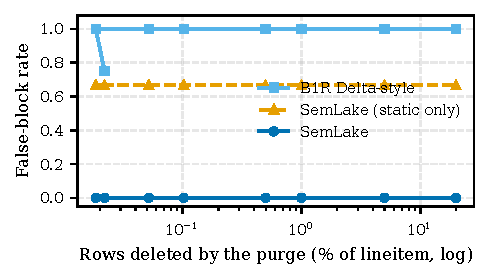
\includegraphics[width=\columnwidth]{figures/fig_selectivity.pdf}
\caption{False-block rate when a purge that removes no row read by Q6 runs next to a Q6 report, against the fraction of \texttt{lineitem} the purge deletes. Each point is \SelTrials\ purges in three clause forms (conjunctive, \texttt{NOT} and \texttt{OR}).}
\label{fig:selectivity}
\end{figure}

\paragraph{Selectivity.} Figure~\ref{fig:selectivity} isolates false blocks. A report reads with Q6's filter, and a purge deletes a random range of part keys restricted to discounts Q6 does not read, so no pair is a true conflict. The purge removes from \SelMinPct\% to \SelMaxPct\% of the table. B1R blocks the report as soon as the purge touches one of the \SelQsixFiles\ files Q6 reads; its false-block rate is \BoneRSelAtOne\ at 0.1\% of rows. The static test alone blocks the \texttt{NOT} and \texttt{OR} forms, a rate of \StaticSelMean. With the row check, \sys\ blocks none.

\subsection{Merge Latency and Requests (Q2)}
\label{sec:eval_scale}

\begin{figure*}[t]
\centering
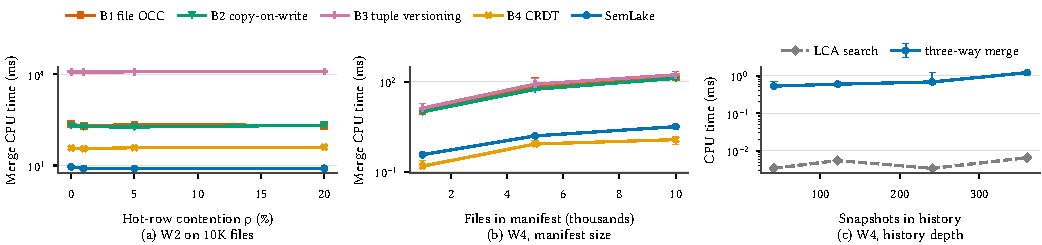
\includegraphics[width=0.95\textwidth]{figures/fig_scalability.pdf}
\caption{Merge CPU time (median of \Repeats\ runs; bars show the range) as (a) hot-row contention grows on a 10K-file table, (b) the manifest grows, and (c) the commit history grows.}
\label{fig:scalability}
\end{figure*}

Figure~\ref{fig:scalability} shows merge CPU time.
\begin{itemize}
  \item \emph{Contention (W2).} On a 10K-file table, \sys\ merges in \WtwoSemZero\,ms at $\kappa = 0$ and \WtwoSemTwenty\,ms at $\kappa = 20\%$, where colliding cells become choices; B1 takes \WtwoBoneZero\,ms and \WtwoBoneTwenty\,ms because it compares full file lists. B4 takes \WtwoBfourZero\,ms at $\kappa = 0$, but it checks nothing: it overwrites one side of every collision.
  \item \emph{Table size (W4).} As the manifest grows from 1K to 10K files, \sys's merge of a schema change and an append takes \WfourSemOne\,ms and \WfourSemTen\,ms. B1, B2 and B3 take \WfourBoneTen\,ms, \WfourBtwoTen\,ms and \WfourBthreeTen\,ms at 10K files; B3 issues \WfourBthreeReq\ requests to rebuild its dictionaries.
  \item \emph{History (W4).} From \HistLow\ to \HistHigh\ snapshots, the LCA search takes \HistLca\,$\mu$s and the merge \HistSemLow\,ms and \HistSemHigh\,ms. Each merge here replays one commit per side, so replay does not explain the growth; the merge also lists the manifest prefix, which grows with the history in our store, and we did not isolate the cause further.
\end{itemize}
CPU time is not the whole story. With the latency model of Section~\ref{sec:impl}, a W2 merge at $\kappa = 0$ is estimated at \WtwoSemEst\,s for \sys\ and \WtwoBoneEst\,s for B1, because \sys\ reads one summary per commit and writes more metadata objects. What \sys\ avoids is growth with table size: on W1 with \WoneSFilesK K files, where each branch updates rows in half of the files, \sys\ issues \WoneSReqSem\ requests (\WoneSPutSem\ \texttt{PUT}, \WoneSGetSem\ \texttt{GET}, \WoneSListSem\ \texttt{LIST}) and writes \WoneSBytesSem\ bytes, while B2 and B3 issue \WoneSReqBtwo\ requests and are estimated at \WoneSBtwoEst\,s. B1 issues only \WoneSReqBone\ requests, but it aborts this merge.

\begin{figure}[t]
\centering
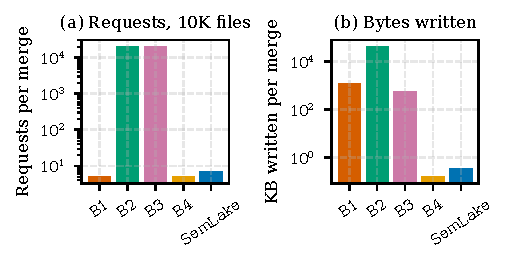
\includegraphics[width=\columnwidth]{figures/fig_requests.pdf}
\caption{Object-store requests and bytes written per W1 merge on a \WoneSFilesK K-file table.}
\label{fig:requests}
\end{figure}

\subsection{Read Overhead and Compaction (Q3)}
\label{sec:eval_read}

\begin{table}[t]
\centering
\footnotesize
\caption{TPC-H Q6 on SF\,1 \texttt{lineitem} after a merge left deletes in a DV: median time of 5 processes, and overhead with a 95\% confidence interval.}
\label{tab:scan}
\setlength{\tabcolsep}{3pt}
\begin{tabular}{@{}l r r r r l@{}}
\toprule
Deletes & Rows & Clean groups & Base (ms) & DV (ms) & Overhead (95\% CI) \\
\midrule
localized & 1\% & 60/61 & 190.5 & 198.2 & +0.9\% ($-$3.4 to +6.9\%) \\
uniform & 0.1\% & 0/61 & 194.0 & 206.8 & +4.2\% ($-$1.7 to +12.5\%) \\
uniform & 1\% & 0/61 & 187.4 & 207.2 & +6.0\% ($-$5.3 to +23.1\%) \\
uniform & 5\% & 0/61 & 178.6 & 187.8 & +5.4\% (+0.2 to +14.2\%) \\
\bottomrule
\end{tabular}
\end{table}


Table~\ref{tab:scan} runs TPC-H Q6 in DuckDB (one thread) over real SF\,1 \texttt{lineitem} (\ScanRows\ rows in \ScanGroups\ row groups of \ScanGroupRows\ rows) after a merge left a DV open. When 1\% of the rows are deleted inside one row group, the overhead is \ScanLocOver\% (95\% CI \ScanLocLow\% to \ScanLocHigh\%). When the same deletes are spread over every row group, every group needs the mask, and the overhead is \ScanUniOver\%. Both intervals are wide relative to the medians: on one thread over SF\,1, the masking cost is small next to the scan itself. The mask is applied by a positional join in our implementation; we did not measure a native DV reader.

\begin{figure}[t]
\centering
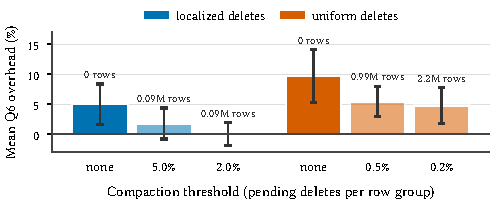
\includegraphics[width=\columnwidth]{figures/fig_compaction.pdf}
\caption{Mean Q6 overhead over \CompMerges\ merges, each deleting \CompDeletePct\% of the rows of SF\,1 \texttt{lineitem}, by compaction threshold (fraction of a row group's rows with pending deletes). Bars show 95\% intervals over the merges; the label above each bar is the number of rows rewritten per merge.}
\label{fig:compaction}
\end{figure}

Figure~\ref{fig:compaction} follows a table through \CompMerges\ merges, each deleting \CompDeletePct\% of its rows, and measures Q6 after every merge. A policy rewrites a row group once the rows deleted in it but still present in its file pass a threshold. Without compaction, the mean overhead is \CompLocNone\% for localized deletes and \CompUniNone\% for uniform ones. With localized deletes, a \CompLocThr\ threshold brings it to \CompLocBest\% and rewrites \CompLocRewrite\ rows per merge, almost one row group. With uniform deletes, the best threshold we tried (\CompUniThr) gives \CompUniBest\% but rewrites \CompUniRewrite\ rows per merge, over a third of the table, because every row group crosses the threshold at about the same time. Per-merge timings vary by more than these differences, so only the means are meaningful. Compaction therefore pays off for localized deletes; for uniform deletes it costs nearly a copy-on-write rewrite to remove a few percent of scan time.

\begin{figure}[t]
\centering
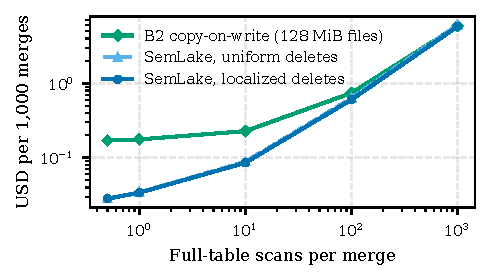
\includegraphics[width=\columnwidth]{figures/fig_cost.pdf}
\caption{Dollars per 1,000 merges (requests, one day of storage for written bytes, and CPU at \$0.10/hour) against the number of full scans per merge, using the overheads of Table~\ref{tab:scan}.}
\label{fig:cost}
\end{figure}

Figure~\ref{fig:cost} combines the measured requests, bytes and overheads into dollars. At 10 scans per merge, 1,000 merges cost \CostSemLoc\ with localized DVs and \CostSemUni\ with uniform ones, against \CostBtwo\ for copy-on-write with 128\,MiB files. Leaving DVs open stays cheaper than rewriting until \CrossLoc\ scans per merge for localized deletes and \CrossUni\ for uniform ones. Past that point the merged files should be compacted.

\subsection{Ablations}
\label{sec:eval_ablation}

\begin{figure}[t]
\centering
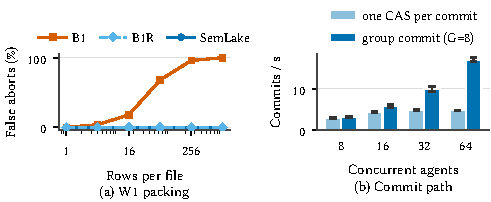
\includegraphics[width=\columnwidth]{figures/fig_ablation.pdf}
\caption{(a) False aborts on W1 as rows per file grow. (b) Swarm commit throughput with one compare-and-swap per commit and with group commit ($G = \SwarmGroup$).}
\label{fig:ablation}
\end{figure}

\paragraph{File packing.} Two branches each update \PackChanged\ random rows of a \PackRows-row table. As rows per file grow from 1 to \PackMax, B1's false-abort rate rises from 0 to \PackBoneMax\ (Figure~\ref{fig:ablation}a). B1R and \sys\ never abort, because both compare rows.

\paragraph{Row check.} Disabling the row check leaves recall unchanged and lowers precision from \SemSuitePrec\ to \StaticSuitePrec\ on the labelled suite and from \SemTpchPrec\ to \StaticTpchPrec\ on the TPC-H pairs; Figure~\ref{fig:selectivity} shows the false blocks it removes.

\paragraph{Replay.} Reading only the tips' summaries loses the predicates of commits merged earlier. The edge-case tests include a report that was merged once before it meets a purge; tip-only replay merges that pair, and Algorithm~\ref{alg:replay} blocks it.

\paragraph{Group commit.} With one compare-and-swap per commit, the swarm of Section~\ref{sec:eval_swarm} reaches \SwarmSemSixtyFour\ commits/s at \SwarmMaxAgents\ agents; with group commit it reaches \SwarmGroupSixtyFour\ (Figure~\ref{fig:ablation}b).

\subsection{Agent Swarm (Q4)}
\label{sec:eval_swarm}

\begin{table}[t]
\centering
\footnotesize
\caption{Simulated swarm, 60\,s per run, mean of 5 seeds ($\pm$ 95\% CI). Haz.: hazards committed and caught, summed over seeds. Blocks and redos: false semantic blocks and false file-conflict redos per run.}
\label{tab:swarm}
\setlength{\tabcolsep}{2.5pt}
\begin{tabular}{@{}r l r r r r r@{}}
\toprule
$N$ & Rule & Commits/s & Haz. & Caught & Blocks & Redos \\
\midrule
8 & B1 file OCC & 1.90 $\pm$ 0.21 & 2 & 0 & 0.0 & 91.4 \\
8 & B1R Delta-style & 2.92 $\pm$ 0.19 & 2 & 2 & 4.8 & 0.0 \\
8 & B2 copy-on-write & 0.65 $\pm$ 0.06 & 0 & 0 & 0.0 & 0.0 \\
8 & \sys & 2.94 $\pm$ 0.16 & 0 & 4 & 0.0 & 0.0 \\
8 & \sys, group commit & 3.18 $\pm$ 0.18 & 0 & 4 & 0.0 & 0.0 \\
\midrule
32 & B1 file OCC & 4.09 $\pm$ 0.11 & 5 & 0 & 0.0 & 488.8 \\
32 & B1R Delta-style & 5.00 $\pm$ 0.04 & 4 & 9 & 19.6 & 0.0 \\
32 & B2 copy-on-write & 1.40 $\pm$ 0.15 & 0 & 0 & 0.0 & 0.0 \\
32 & \sys & 4.86 $\pm$ 0.04 & 0 & 12 & 0.2 & 0.0 \\
32 & \sys, group commit & 10.02 $\pm$ 0.58 & 0 & 19 & 0.2 & 0.0 \\
\midrule
64 & B1 file OCC & 5.02 $\pm$ 0.05 & 20 & 0 & 0.0 & 895.6 \\
64 & B1R Delta-style & 5.13 $\pm$ 0.01 & 11 & 20 & 49.6 & 0.0 \\
64 & B2 copy-on-write & 1.92 $\pm$ 0.25 & 0 & 0 & 0.0 & 0.0 \\
64 & \sys & 4.81 $\pm$ 0.01 & 0 & 43 & 0.4 & 0.0 \\
64 & \sys, group commit & 17.12 $\pm$ 0.40 & 0 & 59 & 1.2 & 0.0 \\
\bottomrule
\end{tabular}
\end{table}


Agent frameworks branch a shared table per agent and merge the results back~\cite{git4data2026,zhou2026chronos}. We simulate this. $N$ agents repeatedly branch from \texttt{main}, work for a random time (mean \SwarmWorkMean\,s), and commit one task: an update of four rows (\SwarmUpdatePct\%), a range delete (\SwarmDeletePct\%) or a report that reads a range and writes an aggregate (\SwarmReportPct\%). The table has \SwarmFiles\ files of \SwarmRowsPerFile\ rows. Publishing is a compare-and-swap with a \SwarmRtt\,ms catalog round trip. The simulation is discrete-event: \sys\ runs on the real engine, and each merge advances simulated time by its measured CPU time plus its counted requests under the latency model; the baselines are rule models charged with the same latency model. A report and a delete that ran concurrently over shared rows are a hazard if both commit. Each run lasts \SwarmHorizon\,s of simulated time. We also run a purge-heavy mix (\SwarmHeavyDeletePct\% deletes, \SwarmHeavyReportPct\% reports) at \SwarmHeavyAgents\ agents; hazard totals below cover both mixes.

Table~\ref{tab:swarm} and Figure~\ref{fig:swarm} give the results. B1 redoes work on every file overlap and B2 rewrites every touched file. B1R and \sys\ both avoid file conflicts, but B1R blocks a report whenever a concurrent delete touched a file it read: \SwarmBoneRFBThirtyTwo\ blocks per run at 32 agents, against \SwarmSemFBThirtyTwo\ for \sys. Over all runs, B1 committed \SwarmBoneHazTotal\ hazards, B2 \SwarmBtwoHazTotal, B1R \SwarmBoneRHazTotal, and \sys\ \SwarmSemHazTotal. B1R still commits hazards because its read check is one-directional: it rejects a report that commits after a delete of rows in files it read, but a delete that commits after the report read nothing the report wrote, so it goes through. With one compare-and-swap per commit, \sys's throughput is limited by the merge's object-store round trips (\SwarmSemSixtyFour\ commits/s at \SwarmMaxAgents\ agents); group commit raises it to \SwarmGroupSixtyFour.

\begin{figure*}[t]
\centering
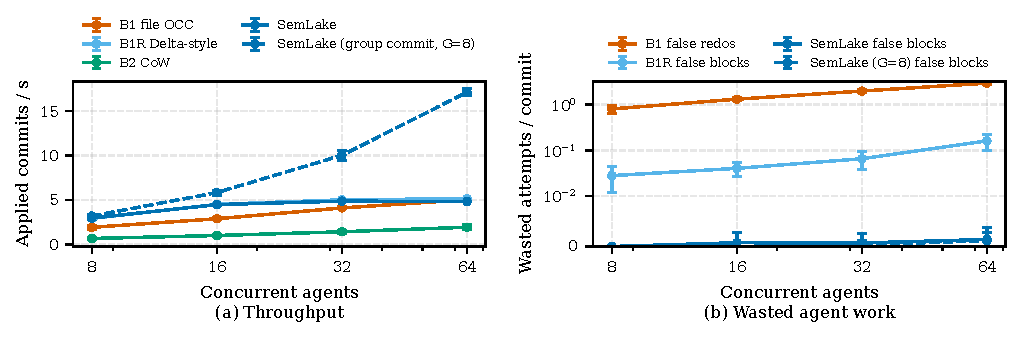
\includegraphics[width=0.95\textwidth]{figures/fig_swarm.pdf}
\caption{Simulated swarm: (a) applied commits per second and (b) wasted attempts per applied commit (false redos for B1, false blocks for B1R and \sys), mean of \SwarmSeeds\ seeds with 95\% confidence intervals.}
\label{fig:swarm}
\end{figure*}

%%%%%%%%%%%%%%%%%%%%%%%%%%%%%%%%%%%%%%%%%%%%%%%%%%%%%%%%%%%%%%%%%%%%%%%%%%%%%%%%
\section{Related Work}
\label{sec:related}

\paragraph{Lakehouse formats and catalogs.} Delta Lake~\cite{armbrust2020delta}, Iceberg~\cite{iceberg2025v3} and Hudi~\cite{jain2023analyzing} add transactions to object-store tables, and their concurrency control compares written files or, in Delta's row-level mode, written rows and read files~\cite{deltaconcurrency}. Deletion vectors and row lineage make row-level changes cheap~\cite{okolnychyi2024petabyte,delta2024rowlevel}. Comparisons of these formats~\cite{jain2023analyzing,camacho2024lstbench} study single-branch workloads. Multi-table transactions~\cite{gotz2026interoperable} and catalog engines~\cite{oh2025treecat} coordinate commits across tables but do not merge branches. lakeFS~\cite{lakefs} and Nessie~\cite{nessie} provide Git-like branches over lakehouse tables and merge them by comparing which objects or tables changed. \sys\ is complementary: it decides whether two branches of one table can be merged, at row and predicate granularity.

\paragraph{Dataset versioning.} DataHub~\cite{bhardwaj2015datahub}, Decibel~\cite{maddox2016decibel}, OrpheusDB~\cite{huang2017orpheusdb}, ForkBase~\cite{wang2018forkbase} and the storage trade-offs of Bhattacherjee et~al.~\cite{bhattacherjee2015principles} focus on storing and retrieving versions. Dolt~\cite{dolt2026} merges cells and checks declared constraints, which we compare against.

\paragraph{Concurrency control.} Predicate locks~\cite{eswaran1976notions} block a write that falls in a range another transaction read, which is the online counterpart of our static test; \sys\ applies the test after the fact, to two finished branches, and adds a check of the deleted rows' values. Adya's dependency graphs~\cite{adya1999weak} and SSI~\cite{cahill2008serializable} define and enforce serializability; Proposition~\ref{prop:serializability} shows why a published merge needs a different invariant. CRDTs~\cite{almeida2024crdt,faria2025crdv} always converge, which on W2 means losing one write.

\paragraph{Program merge.} Verified three-way merge~\cite{sousa2018verified}, version-space representations of conflicts~\cite{zhu2018conflict} and semantic-conflict detection by tests~\cite{dasilva2024detecting} treat merge as a semantic question over programs. \sys\ asks the same question over table predicates and deleted rows.

\paragraph{Agents on shared data.} Git4Data~\cite{git4data2026} and Chronos~\cite{zhou2026chronos} give agents branches over databases. Git4Data names cross-branch semantic conflicts as open; \sys\ is one answer for lakehouse tables.

%%%%%%%%%%%%%%%%%%%%%%%%%%%%%%%%%%%%%%%%%%%%%%%%%%%%%%%%%%%%%%%%%%%%%%%%%%%%%%%%
\section{Limitations and Conclusion}
\label{sec:conclusion}

\paragraph{Limitations.} The prototype runs in one Python process over an in-memory object store; request costs and latencies are modelled, not measured on S3. Scans apply DVs through a Parquet mask and a positional join rather than a native bitmap reader. Compaction and the merge service live in the benchmark harness, compaction was measured on one thread at SF\,1 only, and the swarm is a simulation. B1, B1R, B2 and B6 are rule models of the systems' documented behaviour. The TPC-H pairs use scale factor \TpchSF\ and the read experiments scale factor 1; larger scales were not run. Purge-safety covers deletes, not updates that move rows out of a read range, and a read clause with a join or subquery cannot be checked against rows and is treated as overlapping. Schema widening follows the prototype's list, which includes the lossy integer-to-double case.

\paragraph{Conclusion.} Branch merges in lakehouses are decided today by which files or rows two branches wrote, which both aborts safe merges and accepts unsafe ones. \sys\ decides them from what the branches read and deleted, using summaries that each commit already has to write. A static clause test handles most pairs at once, a check of the deleted rows' values removes the remaining false conflicts, and the merge publishes deletion vectors instead of rewriting files. In our experiments this caught every read--delete hazard, blocked far fewer safe merges than file-granularity read checks, and kept merge requests independent of table size.

\bibliographystyle{ACM-Reference-Format}
\bibliography{references_pvldb}

\end{document}
